\documentclass[tikz,border=5mm]{standalone}
\usepackage{tikz}
\usetikzlibrary{calc,angles,quotes}

\begin{document}
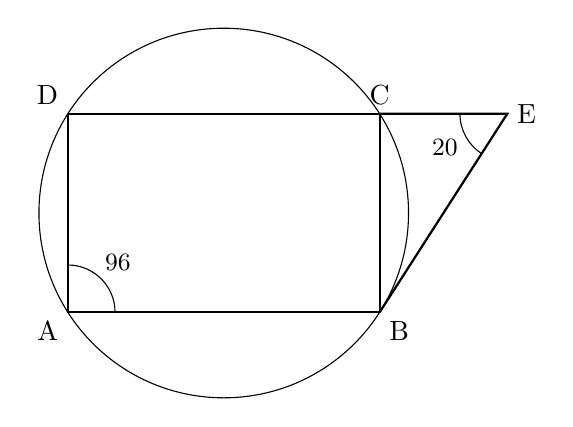
\begin{tikzpicture}[scale=1.8]

% Quadrilateral vertices (cyclic)
\coordinate (A) at (0,0);
\coordinate (B) at (2.2,0);
\coordinate (C) at (2.2,1.4);
\coordinate (D) at (0,1.4);

% Center for circumscribed circle
\coordinate (O) at (1.1,0.7);
\pgfmathsetmacro{\r}{sqrt(1.1*1.1+0.7*0.7)}

% Draw circle
\draw (O) circle (\r);

% Draw quadrilateral ABCD
\draw[thick] (A) -- (B) -- (C) -- (D) -- cycle;

% External point E (on line DC extended)
\coordinate (E) at (3.1,1.4);

% Draw line CE and EB
\draw[thick] (C) -- (E) -- (B);

% 96° angle at A (angle DAB) - INSIDE the quadrilateral
\pic[draw, angle radius=6mm, angle eccentricity=1.5, "$96°$" font=\small] {angle=B--A--D};

% 20° angle at E (angle CEB) - INSIDE (between lines EC and EB)
\pic[draw, angle radius=6mm, angle eccentricity=1.5, "$20°$" font=\small] {angle=C--E--B};

% Vertex labels
\node[below left] at (A) {A};
\node[below right] at (B) {B};
\node[above] at (C) {C};
\node[above left] at (D) {D};
\node[right] at (E) {E};

\end{tikzpicture}
\end{document}